\newpage
\chapter{Implementación del Software}
\vspace{3\baselineskip}

\section{Arquitectura general}
\label{subsec:estructura_arquitectura}

El diseño estructural del software se fundamenta en una separación de responsabilidades, que permite desarrollar y evaluar de forma independiente cada parte del sistema. Con este objetivo, se adoptó el patrón de diseño arquitectónico MVP, el cual divide el sistema en tres capas lógicas bien definidas: la Vista, el Modelo y el Presentador. Esta organización asegura el desacoplamiento de componentes, facilitando la escalabilidad del sistema ante la incorporación de otros modelos de osciloscopios o métodos adicionales de análisis.

La división de tareas facilita la validación algorítmica y control de la incertidumbre matemática especificados en la norma \cite{iec61083_2}, permitiendo someter los algoritmos a ensayos automatizados, aislados de cualquier interfaz gráfica de usuario.

\begin{figure}[H]
    %\centering
    %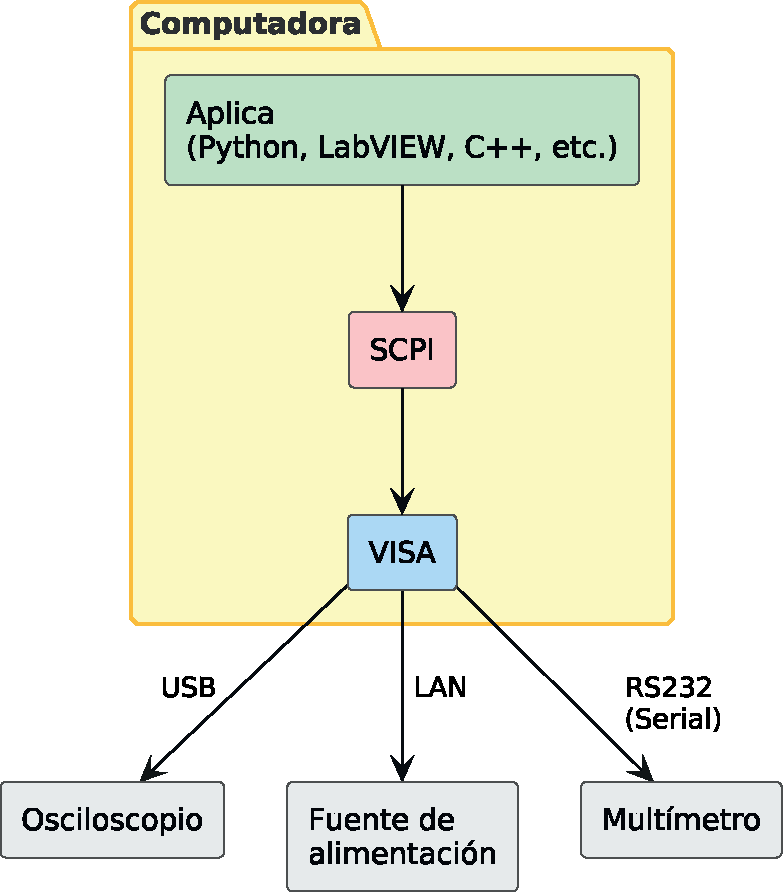
\includegraphics{img/arquitectura_instrumentacion.pdf}
    \caption{Diagrama de bloque de la arquitectura.}
    \label{fig:Lab_1_Circ_1_V1-esquema}
\end{figure}

\subsection{Capa de Presentación: Vista}
\label{subsec:vista}

La \textbf{Vista} maneja de forma exclusiva la representación visual del sistema y la captura de las interacciones del operador. Ya que, solo declara estáticamente la disposición y propiedades de los componentes gráficos.

Esta capa se caracteriza por no tener referencias directas hacia la lógica de adquisición física o los algoritmos de procesamiento digital de señales. Ante cualquier interacción física del usuario, como el accionamiento de botones o la inserción de datos, la Vista emite eventos en forma de señales de Qt (\textbf{Qt Signals}), que son interceptadas por el Presentador para desencadenar el flujo correspondiente.

\subsection{Capa de Lógica y Datos: Modelo}
\label{subsec:modelo}

El \textbf{Modelo} representa el núcleo funcional del software, abarcando el control del instrumental de laboratorio, la lógica de cálculo metrológico y la administración de la persistencia de datos.

Esta capa se subdivide en tres submódulos independientes especializados:

\begin{enumerate}
    \item \textbf{Abstracción de Hardware}: Implementada en el módulo \textbf{GWInstekGDS1000AU}. Encapsula todas las operaciones de control, configuración de canales y adquisición de datos de la memoria del osciloscopio, mediante comandos SCPI, usando el protocolo de comunicación PyVISA.
    \item \textbf{Persistencia y Gestión de Archivos}: Administrada por el módulo \textbf{FileManager}. Maneja la creación y el acceso al sistema de archivos. Su función principal es el almacenamiento en bases de datos utilizando el formato HDF5. Asimismo, gestiona la exportación de resultados a hojas de cálculo tipo CSV o XLSX.
    \item \textbf{Procesamiento Digital de Señales}: Llevado a cabo por el módulo matemático \textbf{LightningImpulseAnalyzer}. Constituye el motor matemático del sistema. Es responsable de acondicionar la señal y extraer sus parámetros característicos según la norma \cite{iec60060_1}.
\end{enumerate}

\subsection{Capa de Coordinación: Presentador}
\label{subsec:presentador}

El \textbf{Presentador}, es implementado en el módulo \textbf{MainPresenter}, y actúa como coordinador de la arquitectura MVP. Tiene como responsabilidad orquestar la interacción entre la interfaz visual y los motores lógico-físicos.

\section{Controlador de \emph{hardware}}
\label{sec:controlador_osciloscopio}

En esta sección se expone la implementación controlador del osciloscopio, cuya función general es abstraer las operaciones de bajo nivel, permitiendo desacoplar la comunicación con el dispositivo del resto del sistema.

\subsection{Interfaz de comunicación y capa de abstracción de hardware}
\label{subsec:interfaz_fisica_hal}

A nivel de \emph{software}, para evitar el acoplamiento directo del código de la aplicación con las llamadas al sistema de bajo nivel (capa física de transmisión), se implementa una Capa de Abstracción de Hardware (HAL, \emph{Hardware Abstraction Layer}), bajo la Arquitectura VISA. Esta capa de abstracción permite que los comandos de consulta (\textit{queries}) y configuración (\textit{writes}) permanezcan independientes de la interfaz de hardware utilizada (sea USB, GPIB, Ethernet o RS-232), permitiendo actualizaciones de la instrumentación sin necesidad de modificar el código del presentador.

El controlador inicializa el administrador de recursos, y ejecuta un escaneo automático para buscar algún dispositivo conectado, que tenga un descriptor de recurso lógico VISA, como el siguiente:
\begin{align*}
    \texttt{ASRL1::INSTR}
\end{align*}

Si encuentra al menos un dispositivo direccionable, se conecta al mismo. La comunicación inicia instanciando el administrador de recursos VISA de Python (PyVISA), acompañado de la biblioteca \texttt{pyvisa-py} para asegurar un entorno multiplataforma sin depender de bibliotecas nativas propietarias.

Sobre el canal de transporte establecido con VISA, el software envía comandos SCPI, que debe cumplir con el siguiente formato indicado en el manual del fabricante \cite{gds1000au_ProgrammingManual}:
\begin{itemize}
    \item \textbf{No sensibilidad a mayúsculas:} Puede usarse mayúsculas y minúsculas.
    \item \textbf{Separación de parámetros:} Al configurar parámetros, debe separarse el comando y su argumento numérico, mediante un carácter de espacio en blanco simple.
    \item \textbf{Finalizador de mensaje:} Cada instrucción enviada al osciloscopio debe finalizar con el carácter delimitador de fin de mensaje \emph{Line Feed} (\textbf{\texttt{LF}}, en hexadecimal \textbf{\texttt{0x0A}} o a la secuencia de escape \textbf{\texttt{\textbackslash n}}), para que el instrumento proceda a interpretar y ejecutar la orden.
\end{itemize}

Para gestionar la configuración del osciloscopio de manera robusta, se implementa una arquitectura, basada en métodos de consulta (\emph{getters}) y configuración (\emph{setters}), que encapsulan los comandos SCPI.

Los métodos de consulta usan la instrucción \textbf{\texttt{.query()}}, reciben una cadena de caracteres, que deben convertir al tipo de dato correspondiente (\texttt{float}, \texttt{int} o \texttt{string}) y la retornan al presentador. En tanto que, los métodos de configuración emplean la instrucción \textbf{\texttt{.write()}}, sin esperar ninguna respuesta del instrumento.

Este flujo se protege con una rutina de control de excepciones que, ante fallos críticos en el bus o pérdidas de sincronismo, aborta la operación y libera los recursos del sistema de forma segura, ya que de lo contrario impediría la reconexión posterior del instrumento, debiendo reiniciar la computadora o el osciloscopio.

A continuación, se ejemplifican los métodos de consulta y configuración de la escala vertical de un canal.
\begin{python}
# Método de consulta.
def get_channel_scale(channel):
    scale = dso.query(f':channel{channel}:scale?')
    v_scale = float(scale)
    return v_scale

# Método de configuración.
def set_channel_scale(channel, value):
    dso.write(f':channel{channel}:scale {value}')
\end{python}

Por otro lado, a nivel físico, la conexión se realiza a través de un puerto USB 2.0 tipo B (esclavo) ubicado en el panel posterior del instrumento, y un puerto USB tipo A (maestro) de la computadora. Aunque, si bien el equipo se conecta a través de un puerto USB, la computadora lo detecta como un dispositivo de comunicación serie virtual\footnote{El controlador (\emph{driver}) USB, está disponible en la página del fabricante \cite{gds1000au_driver}.}, bajo la Clase de Dispositivo de Comunicación con Modelo de Control Abstracto (CDC-ACM, \emph{Communication Device Class - Abstract Control Model}), que aparece en el administrador de dispositivos con el siguiente nombre \cite{gds1000au_ProgrammingManual}:
\begin{align*}
    \texttt{COM1}
\end{align*}
Donde \texttt{COM1} identifica el número de puerto serie virtual asignado por el sistema operativo.

\subsection{Sistema de Adquisición y Almacenamiento}
\label{subsec:arquitectura_flujo}

La adquisición del impulso de alta tensión desde el generador Marx, hasta el almacenamiento en la computadora, se estructuran de la siguiente forma:

\begin{enumerate}
    \item Acondicionamiento analógico.
    \item Captura de impulso
    \item Digitalización.
    \item Desempaquetado de datos.
    \item Reconstrucción y escalamiento de la onda.
\end{enumerate}

\subsubsection{Acondicionamiento analógico}

La señal eléctrica, debe ser adaptada en amplitud antes de ingresar al osciloscopio, para no dañarlo.

Para el canal de tensión (CH1), la señal se deriva utilizando un divisor de tensión resistivo, acoplado en cascada serie con un atenuador coaxial, por lo que el factor de atenuación equivalente resulta:
\begin{equation}
    \label{eq:atenuacion_tension}
    A_{\text{CH1}} = \text{Divisor} \times \text{Atenuador}
\end{equation}

Para el canal de corriente (CH2), la descarga atraviesa una resistencia shunt conectada en serie con el elemento bajo ensayo, de la cual se toma su tensión a bornes, acoplada a un atenuador que reduce su magnitud a niveles adecuados.
\begin{equation}
    \label{eq:atenuacion_corriente}
    A_{\text{CH2}} = R_\text{Shunt} \times \text{Atenuador}
\end{equation}

Ambas señales llegan al instrumento por medio de cables coaxiales de \qty{50}{\ohm}, para reducir acoplamientos electromagnéticos parásitos (EMI).

\subsubsection{Captura de impulso}
\label{subsec:captura_impulso}

La captura de impulsos (\qty[parse-numbers=false]{1.2/50}{\micro\second}) requiere que el osciloscopio opere en modo de disparo único (\emph{Single Trigger}), dado que es un transitorio no periódico.

Cuando el operador inicia el modo de captura desde la GUI, el presentador crea y ejecuta un subproceso asíncrono, que mediante el controlador de \emph{hardware}, realiza un sondeo periódico (\emph{polling}) al osciloscopio, para saber el estado de disparo del mismo.

Al detectar el impulso finaliza el bucle de \emph{polling} y emite una señal, que es capturada en el hilo de ejecución principal por un receptor (\emph{slot}) del presentador, y finaliza el subproceso.

Como el instante de descarga es indeterminado, se implementa un hilo de ejecución secundario asíncrono, dedicado a consultar el estado de disparo, ya que si se ejecutara en el hilo principal, sería una operación bloqueante, que congele la aplicación e inhabilite la GUI. Por lo que, así se mantiene siempre reactivo el hilo principal de eventos gráficos, permitiendo al usuario manipular oscilogramas previos, cargar campos o cualquier otra acción, mientras el sistema espera la captura del impulso.

\subsubsection{Digitalización}

Las señales eléctricas que ingresan a los bornes analógicos del osciloscopio, se muestrean a una tasa que depende de la base de tiempo utilizada. Después, el convertidor analógico-digital (ADC) realiza la cuantización en amplitud, dividiendo el rango dinámico vertical en $2^8 = 256$ niveles de tensión discretos (\num{8} bits). A continuación, se graban en la memoria del instrumento.

\subsubsection{Desempaquetado de datos}
\label{subsec:desempaquetado_datos}

Luego de que el osciloscopio digitalice la señal, el presentador ordena la descarga de los datos brutos (\emph{RAW}) de los canales habilitados, y recibe un bloque de datos, compuestos por el encabezado y el vector de datos de la onda, que cumple con la siguiente estructura\footnote{La estructura de datos descrita en el manual del fabricante tiene algunas diferencias con los resultados obtenidos del instrumento, debido a la dificultad que esto presentó al momento de intentar procesarla, se contactó con el frabricante obteniendo un script de procesamiento del paquete de datos, que se corresponde con el formato indicado en este trabajo. A su vez, se encontró que el manual de programación de la series GDS-1000B aporta detalles explicativos sobre cómo procesar esta estructura \cite{gds1000b_ProgrammingManual}} \cite{gds1000au_ProgrammingManual}:

\begin{equation*}\label{eq:formato_memoria}
\text{\texttt{\# A B C D E}}
\end{equation*}
\begin{enumerate}
    \item[\texttt{\#:}] [\num{1} byte] Caracter ASCII que indica el inicio de la cabecera.
    \item[\texttt{A:}] [\num{1} byte] Dígito ASCII que especifica la cantidad de caracteres que componen el campo \texttt{B}. Para adquisiciones estándar toma el valor ASCII \texttt{'4'}, mientras que para adquisiciones de memoria extendida toma el valor \texttt{'7'}.
    \item[\texttt{B:}] [\num{4} o \num{7} bytes] Cadena de caracteres ASCII que representa el tamaño total en bytes del bloque de datos que le sigue (\texttt{C}+\texttt{D}+\texttt{E}).
    Para adquisiciones estándar toma el valor ASCII \texttt{'8008'}, mientras que para adquisiciones de memoria extendida puede tomar los valores \texttt{'2000008'} o \texttt{'4000008'}.
    \item[\texttt{C:}] [\num{4} bytes] Intervalo de tiempo ($\Delta t$) entre dos muestras consecutivas de la señal, en formato de punto flotante de precisión simple según IEEE-754 (\num{32} bits), en orden \emph{little-endian} (se envía primero el byte menos significativo):
    \begin{equation*}\label{eq:periodo_muestreo}
    \Delta t = t[n+1] - t[n]
    \end{equation*}
    \item[\texttt{D:}] [\num{4} bytes] Bloque de datos no utilizado.
    \item[\texttt{E:}] [\num{8e3}, \num{2e6} o \num{4e6} bytes] Vector de datos de la onda, cuya longitud es definida en el campo \texttt{B}. Cada valor entero (base \num{10}) es expresado con \num{2} bytes (\num{16} bits), y transmitidos en orden \emph{big-endian} (se envía primero el byte más significativo).
\end{enumerate}

Una vez finalizada la descarga de datos, el presentador ordena al controlador de \emph{hardware} que decodifique cada bloque acorde a su formato, considerando la estructura recién mencionada.

\subsubsection{Reconstrucción y escalamiento de la onda}

Con el vector de valores enteros brutos decodificado, primero se aplica la ecuación \eqref{eq:reconstruccion_tension} para reconstruir la forma de onda que llegó a bornes del osciloscopio, considerando la escala vertical configurada al momento de la captura, y el Factor AD = \num{25} definido en el manual de programación del fabricante \cite{gds1000au_ProgrammingManual}:
\begin{equation}
\label{eq:reconstruccion_tension}
\text{Onda sin escalar}[n] = \text{Datos brutos}[n] \times \frac{{\text{V/div}}}{\text{Factor AD}}
\end{equation}
A continuación, para obtener las magnitudes reales aplicadas al objeto bajo ensayo, se multiplica escalarmente los vectores de tensión y corriente, por sus respectivos factores de atenuación, cargados por el usuario en los campos pertinentes de la ventana, aplicando la siguiente ecuación:
\begin{equation}
\label{eq:reconstruccion_tension_total}
{\text{Onda escalada}}[n] = \text{Onda sin escalar}[n] \times A_{\text{CH<X>}}
\end{equation}
Los vectores resultantes de tensión (en volts, \unit{\volt}) y de corriente (en amperes, \unit{\ampere}), se transfieren al módulo de procesamiento matemático para determinar sus parámetros normativos: tiempo de frente $T_1$, tiempo de cola $T_2$, valor de cresta $U_{\text{t}}$ y sobreimpulso OS, conforme a los requerimientos de la norma \cite{iec60060_1}.

\section{Motor de Cálculo: Procesamiento de Señales y Ajuste de Curvas}
\label{sec:motor_calculo}

Este componente constituye el núcleo matemático del software, y es responsable de obtener los parámetros normativos a partir de los arreglos temporales de tensiones discretas adquiridas por el \emph{hardware}.

El motor de cálculo ha sido diseñado exclusivamente para cumplir con las normas IEC 60060-1 \cite{iec60060_1} e IEC 61083-2-1 \cite{iec61083_2}, aplicando criterios de modularidad, que permiten su validación automatizada e independiente del resto de la aplicación.

\subsection{Flujo algorítmico de cálculo}
\label{sec:flujo_algoritmico}

Este proceso se divide en tres fases operativas: preprocesamiento común, clasificación dinámica y reconstrucción de la señal.

\subsubsection{Fase I: Acondicionamiento Inicial}

Esta etapa es común a todos los registros adquiridos.
\begin{enumerate}
    \item \textbf{Eliminación de offset}: Se calcula el valor de tensión continua ($V_{\text{offset}}$) promediando estadísticamente una ventana de datos adquiridos ($N_{\text{pretrigger}}$) en el instante previo al disparo (``pre-trigger''), donde la curva registrada ($U_\text{e}[n]$) es nula.
    \begin{equation}
        \label{eq:calculo_offset}
        V_{\text{offset}} = \frac{1}{N_{\text{pretrigger}}} \sum_{n=1}^{N_{\text{pretrigger}}} U_\text{e}[n]
    \end{equation}
    El vector de tensión corregida se calcula como:
    \begin{equation}
        \label{eq:eliminacion_offset}
        U_{\text{corregida}}[n] = U_\text{e}[n] - V_{\text{offset}}
    \end{equation}
    \item \textbf{Normalización de polaridad}: Dado que los impulsos pueden ser de polaridad positiva o negativa, el algoritmo detecta el sentido del impulso evaluando el signo de la muestra extrema:
    \begin{equation}
        \label{eq:buscar_polaridad}
        \text{polaridad} = \text{sign}(\text{arg max} |U_{\text{corregida}}[n]|)
    \end{equation}
    El vector de tensión corregida se multiplica por este término para simplificar el resto del procesamiento, asegurando que el análisis sea exclusivamente en el semiplano positivo:
    \begin{equation}
        \label{eq:normalizacion_polaridad}
        U_{\text{abs}}[n] = \text{polaridad} \cdot U_{\text{corregida}}[n]
    \end{equation}
    \item \textbf{Normalización unitaria}: Se normaliza la amplitud al dominio unitario respecto a su valor de cresta.
    \begin{equation}
        \label{eq:onda_normalizada}
        U_{\text{norm}}[n] = \frac{U_{\text{abs}}[n]}{\max(U_{\text{abs}}[n])}
    \end{equation}
\end{enumerate}

\subsubsection{Fase II: Bifurcación de análisis e identificación de parámetros base}

En este punto, el flujo se divide según si debe procesar un impulso de referencia (pleno) o un impulso de ensayo, que puede ser pleno o cortado.

\textbf{Caso A: Análisis de impulso de referencia (pleno)}

Se asume que la onda es plena y se procede al ajuste paramétrico.
\begin{enumerate}[resume]
    \item \textbf{Segmentación de datos}: Se selecciona una ventana de datos en el intervalo comprendido entre el \qty{20}{\percent} en el flanco de subida y el \qty{40}{\percent} en la cola de descarga del impulso.
    \item \textbf{Ajuste de curva base}: Se realiza un ajuste paramétrico no lineal sobre la ventana de muestras, utilizando el algoritmo de \textbf{Levenberg-Marquardt}, teniendo como modelo de estimación la función de doble exponencial:
    \begin{equation}
        \label{eq:modelo_doble_exponencial}
        u_d[n] = U \cdot \left( e^{-\frac{t - t_d}{\tau_1}} - e^{-\frac{t - t_d}{\tau_2}} \right)
    \end{equation}
    Donde los coeficientes desconocidos a determinar son:
    \begin{itemize}
        \item $U$ el parámetro de amplitud escalar.
        \item $\tau_1$ la constante de tiempo de descarga.
        \item $\tau_2$ la constante de tiempo de carga.
        \item $t_d$ el retardo temporal del origen virtual.
    \end{itemize}
\end{enumerate}

\textbf{Caso B: Análisis de ensayo (LI vs. LIC)}

Si evalúa una onda de ensayo, se inyectan los parámetros de la onda de referencia procesada en el \textbf{Caso A}, y se ejecuta el siguiente análisis:
\begin{enumerate}[resume]
    \item \textbf{Cálculo del desfasaje temporal}: El corrimiento temporal, $t_L$, entre el frente de onda del último impulso con el de referencia, se calcula como el promedio de las diferencias de los instantes de tiempo, correspondientes al \qty{30}{\percent}, \qty{50}{\percent} y \qty{80}{\percent} de $U_\text{t}$ respectivamente, de ambos impulsos.
    \begin{equation}
        t_L = \frac{\left( t_{30, \text{ref}} - t_{30, \text{i}} \right) + \left( t_{50, \text{ref}} - t_{50, \text{i}} \right) + \left( t_{80, \text{ref}} - t_{80, \text{i}} \right)}{3} 
    \end{equation}
    \item \textbf{Alineación del eje temporal}: Se obtiene el vector temporal alineado del impulso de ensayo, $t_\text{aligned}[n]$, partiendo de su vector temporal original $t[n]$, al que se lo desplaza la cantidad $t_L$.
    \begin{equation}
        \label{eq:eje_alineado}
        t_\text{aligned}[n] = t[n] + t_L
    \end{equation}
    \item \textbf{Clasificación del impulso}: Se calcula la diferencia absoluta punto a punto entre el impulso de ensayo y el de referencia, usando sus vectores normalizados en amplitud.
    \begin{equation}
        \label{eq:umbral_desviacion}
        | U_{\text{norm, i}}[n] - U_{\text{norm, ref}}[n] | > umbral
    \end{equation}
\end{enumerate}

En caso de que la desviación no supere el umbral, la onda es clasificada como \textbf{impulso pleno (LI)} y el flujo se dirige al \textbf{Caso A}.

Si la desviación supera el umbral, la onda se clasifica como \textbf{impulso cortado (LIC)} y se procede a analizar el colapso de la onda.
\begin{enumerate}[resume]
    \item \textbf{Cálculo del factor de escala}: Se calcula como el promedio del intervalo comprendido entre el \qty{30}{\percent} y \qty{80}{\percent} de $U_{\text{corregida}}[n]$ del frente de la onda de ensayo y la de referencia.
    \begin{equation}
        \overline{U_\text{i}} = \frac{1}{N} \sum_{n = k_{30\%}}^{k_{80\%}} U_\text{i}[n]
    \end{equation}
    \begin{equation}
        \overline{U_\text{ref}} = \frac{1}{N} \sum_{n = k_{30\%}}^{k_{80\%}} U_\text{ref}[n]
    \end{equation}
    \begin{equation}
        \label{eq:factor_escala_e}
        E = \frac{\overline{U_\text{i}}}{\overline{U_\text{ref}}}
    \end{equation}
    \item \textbf{Escalado de la curva base}: Debido a que la descarga disruptiva hace colapsar el ajuste por el corte abrupto de la señal, se sintetiza la curva base de la onda de referencia $U_\text{b, ref}[n]$, y se escala en amplitud con el factor de escala $E$.
    \begin{equation}
        \label{eq:curva_base_lic}
        U_\text{b, i}[n] = E \cdot U_\text{b, ref}[n]
    \end{equation}
    \item \textbf{Tiempo de corte}: Se analiza la cola del impulso, minimizando la derivada primera para localizar el sector de máxima pendiente de caída:
    \begin{equation}
        \label{eq:gradiente_colapso}
        n_\text{abrupto} = \text{arg min}\left(\frac{\text{d} U_{\text{cola}}[n]}{\text{d} t}\right)
    \end{equation}
    El inicio del colapso se encuentra evaluando el punto de inflexión local mediante la derivada segunda:
    \begin{equation}
        \label{eq:punto_inflexión}
        n_\text{inflexion} = \text{arg min}\left(\frac{\text{d}^2 U_\text{cola}[n]}{\text{d}^2 t}\right)
    \end{equation}
    Con ese índice se obtiene la tensión del colapso:
    \begin{equation}
        U_\text{colapso} = U_\text{corregida}[n_\text{pico} + n_\text{inflexion}]
    \end{equation}
    Se calculan los instantes correspondientes al \qty{70}{\percent} y al \qty{10}{\percent} de $U_\text{colapso}$ sobre el flanco descendente, para extrapolar linealmente el instante de corte, para el nivel de $U_{\text{colapso}}$:
    \begin{equation}
        t_c = t_{70} + (U_{\text{colapso}} - U_{70}) \left(\frac{t_{10} - t_{70}}{U_{10} - U_{70}}\right)
    \end{equation}
    Finalmente, se calcula el tiempo de corte respecto al origen virtual:
    \begin{equation}
        T_c = t_c - O_1
    \end{equation}
\end{enumerate}

\subsubsection{Fase III: Convergencia, Filtrado y Parámetros Característicos}

Independientemente de la ruta ejecutada en la Fase II, el algoritmo converge obteniendo una curva registrada y una curva base (ajustada numéricamente o escalada analíticamente), para avanzar a la secuencia final:
\begin{enumerate}[resume]
    \item \textbf{Cálculo de curva residual}: Se obtiene como la diferencia algebraica entre la curva corregida ($U_{\text{corregida}}[n]$) y la curva base ($U_\text{b}[n]$) construída con los parámetros obtenidos del ajuste:
    \begin{equation}
        \label{eq:curva_residual}
        R[n] = U_{\text{corregida}}[n] - U_\text{b}[n]
    \end{equation}
    \item \textbf{Filtrado digital de fase cero}: 
    Se obtiene la curva residual filtrada ($R_f[n]$), aplicando un filtro digital IIR a la curva residual ($R[n]$). Para reducir el ruido de muy alta frecuencia relacionado a la interferencia electromagnética, sin perder oscilaciones propias del ensayo.
    \item \textbf{Curva de tensión de ensayo}: Se sintetiza la curva de ensayo ($U_\text{t}[n]$) sumando algebraicamente la curva base analítica con la residual filtrada:
    \begin{equation}
        \label{eq:curva_ensayo}
        U_\text{t}[n] = U_\text{b}[n] + R_f[n]
    \end{equation}
    \item \textbf{Cálculo de parámetros característicos}: A partir de la curva de tensión de ensayo $U_\text{t}[n]$, se calculan los parámetros normativos. Dado que la señal procesada es de tiempo discreto, hay valores analíticos que pueden no corresponder con las muestras obtenidas, por lo que para encontrarlos se realiza una interpolación lineal.
    \begin{itemize}
        \item \textbf{Valor de cresta} ($U_\text{t}$): Es la amplitud máxima de la curva de tensión de ensayo $U_\text{t}[n]$:
        \begin{equation}
            \label{eq:valor_cresta}
            U_\text{t} = \text{max}(U_\text{t}[n])
        \end{equation}
        \item \textbf{Tiempo de frente} ($T_1$): Se calcula como el cociente del intervalo temporal transcurrido entre los instantes $t_{30}$ y $t_{90}$ (correspondientes al \qty{30}{\percent} y \qty{90}{\percent} de $U_\text{t}$ respectivamente), dividido por $\num{0.6}$:
        \begin{equation}
            \label{eq:tiempo_frente}
            T_1 = \frac{t_{90} - t_{30}}{\num{0.6}}
        \end{equation}
        \item \textbf{Origen virtual} ($O_1$): El inicio ficticio de la descarga eléctrica se calcula:
        \begin{equation}
            \label{eq:origen_virtual}
            O_1 = t_{30} - \num{0.5} \cdot (t_{90} - t_{30})
        \end{equation}
        \item \textbf{Tiempo de cola} ($T_2$): El intervalo temporal entre el origen virtual $O_1$ y el instante $t_{50}$, correspondiente al \qty{50}{\percent} de $U_\text{t}$ en el flanco descendente de la onda, se calcula:
        \begin{equation}
            \label{eq:tiempo_cola}
            T_2 = t_{50} - O_1
        \end{equation}
        \item \textbf{Sobreimpulso relativo} ($\text{OS}\%$): Se calcula como la diferencia entre el valor extremo de la curva registrada ($U_\text{e}$):
        \begin{equation}
            \label{eq:max_curva_registrada}
            U_\text{e} = \max(U_\text{e}[n])
        \end{equation}
        y el valor máximo de la curva base ($U_\text{b}$):
        \begin{equation}
            \label{eq:max_curva_base}
            U_\text{b} = \max(U_\text{b}[n])
        \end{equation}
        expresado en porcentaje:
        \begin{equation}
            \label{eq:sobreimpulso_relativo}
            \text{OS}\% = \frac{U_\text{e} - U_\text{b}}{U_\text{e}} \cdot \num{100}
        \end{equation}
    \end{itemize}
\end{enumerate}



\noindent
========================================================================

\begin{forest}
  for tree={
    folder,
    grow'=0,
    font=\sffamily\small,
    inner sep=3pt,
    s sep=3pt,        % Separación vertical ajustada
    draw=black!20,    % Color del borde del nodo (opcional)
    fill=black!5,     % Color de fondo del nodo (opcional)
    rounded corners   % Bordes redondeados (opcional)
  }
  [\textbf{Grupo raíz (Archivo .h5)}
    [\textbf{Atributos globales}: \emph{Datos comunes a todos los registros}
      [{\textbf{\texttt{Item}}: \emph{Identificador del objeto a ensayar}}]
      [{\textbf{\texttt{Cliente}}: \emph{Nombre de la entidad solicitante}}]
      [{\textbf{\texttt{Atenuaciones}}: \emph{Factores de atenuación de CH1 y CH2}}]
    ]
    [{\textbf{Grupos de ondas} \emph{Impulso capturado} (\texttt{Onda\_n} / \texttt{Referencia\_n})}
      [\textbf{Atributos particulares}: \emph{Metadatos propios de cada impulso}
        [{\textbf{\texttt{Fecha}}: \emph{Marca de tiempo de adquisición}}]
        [{\textbf{\texttt{Temperatura}}: \emph{Parámetro ambiental}}]
        [{\textbf{\texttt{Humedad}}: \emph{Parámetro ambiental}}]
        [{\textbf{\texttt{Presión}}: \emph{Parámetro ambiental}}]
        [{\textbf{\texttt{Polaridad}}: \emph{Sentido eléctrico del impulso} (+/-)}]
        [{\textbf{\texttt{Valor\_pico}}: \emph{Tensión de cresta}}]
        [{\textbf{\texttt{T1}}: \emph{Tiempo de frente}}]
        [{\textbf{\texttt{T2}}: \emph{Tiempo de cola}}]
        [{\textbf{\texttt{OS}}: \emph{Sobreimpulso porcentual}}]
      ]
      [{\textbf{Grupo de Tiempos} (\texttt{/Time}) [\unit{\second}]}
        [{\textbf{\texttt{raw}}: \emph{Vector bruto a apartir de} $\Delta t$}]
        [{\textbf{\texttt{alineado}}: \emph{Vector alineado con el frente del impulso de referencia}}]
      ]
      [{\textbf{Grupo de CH1} (\texttt{/CH1\_Voltage}) [\unit{\volt}]}
        [{\textbf{\texttt{raw}}: \emph{Vector de tensión bruta, magnitud real}}]
        [{\textbf{\texttt{ensayo}}: \emph{Vector de tensión de ensayo IEC 60060-1}}]
        [{\textbf{\texttt{normalizado}}: \emph{Vector normalizado} ($V_{\text{pico}} = \num{1.0}$)}]
      ]
      [{\textbf{Grupo de CH2} (\texttt{/CH2\_Current}) [\unit{\ampere}]}
        [{\textbf{\texttt{raw}}: \emph{Vector de corriente bruta, magnitud real}}]
        [{\textbf{\texttt{ensayo}}: \emph{Copia del bruto (simetría de procesamiento con CH1)}}]
        [{\textbf{\texttt{normalizado}}: \emph{Vector normalizado} ($I_{\text{pico}} = \num{1.0}$)}]
      ]
    ]
  ]
\end{forest}


\section{Gestión de problemas}
\label{subsec:gestion_fallos}

Para garantizar el funcionamiento continuo y evitar comportamientos indeterminados, ante perturbaciones o errores operativos, la aplicación tiene la siguiente estructura de manejo de problemas:

\begin{enumerate}
    \item \textbf{Errores de comunicación del hardware:} 
    En caso de una desconexión accidental del cable USB, o fallos de alimentación del osciloscopio durante el ensayo, la capa lógica interrumpe la ejecución, emite una notificación al operador sobre la pérdida de comunicación, y reestablece los controles de la interfaz gráfica.
    
    \item \textbf{Validación de datos de entrada:}
    Para impedir que el software realice cálculos numéricos con buffers vacíos o configuraciones incompletas, el presentador realiza validaciones lógicas antes de interactuar con el módulo de almacenamiento o el analizador matemático, previniendo las siguientes fallas:
    \begin{itemize}
        \item \textbf{Ensayo nulo:} Si el operador acciona el botón de \enquote{Guardar} o \enquote{Exportar} sin haber creado previamente la carpeta del ensayo, se detiene la operación, y se notifica la ausencia del directorio del ensayo.
        \item \textbf{Ausencia de condiciones ambientales:} Se restringe el ingreso de datos inválidos en estos campos, y se impide el almacenamiento de la onda si no están cargados, advirtiendo al operador que debe completarlos.
        \item \textbf{Buffer de adquisición vacío:} Si el operador solicita guardar datos sin haber capturado una señal, se interrumpe la escritura de un registro nulo, y genera una alerta de buffer vacío.
    \end{itemize}

    \item \textbf{Fallos del módulo matemático:}
    Durante el procesamiento de la señal, pueden presentarse divergencias o inestabilidades numéricas. En ese caso, el motor de cálculo detiene el proceso, y notifica al operador sobre la necesidad de repetir la captura y reajustar la configuración del oscilocopio (si es necesario).
\end{enumerate}


La etapa 1 de acondicionamiento analógico, es propia del montaje del ensayo, por lo que, no se afecta en ningún aspecto. La etapa 2 de digitalización, se modificó para este proyecto respecto al montaje vigente, analizando entre las alternativas de osciloscopio disponibles en el laboratorio, cuál era el más indicado tanto por sus características eléctricas, como por su capacidad de comunicación con la PC. Mientras que, las etapas 3, 4 y 5 son desarrollo íntegro del presente trabajo.

